\chapter{Τεχνολογιές}

\section{Εισαγωγή}

Αρχικά δημιουργήθηκε η βασική δομή και η δομή της διαδικτυακής πύλης καθορίστηκε. Αυτή η βασική δομή φαίνεται στο Παρακάτω σχήμα

Είναι σημαντικό να σημειωθεί ότι ολόκληρη η εφαρμογή Django βρίσκεται στον ίδιο φυσικό
διακομιστή. Όταν ο χρήστης στέλνει ένα αίτημα για την εκτέλεση ενός σεναρίου με συγκεκριμένες εισόδους αυτό στέλνεται στις συσκευές στο τοπικό δίκτυο.


Το πρώτο βήμα στη διαδικασία ήταν να καθοριστεί τι θα αυτοματοποιηθεί με βάση τις
διάφορες εκτιμήσεις. Για να καθοριστεί αυτό, πραγματοποιήθηκαν πολλές συναντήσεις καταιγισμού ιδεών.
με την ομάδα. Προτού γίνει αυτό όμως η αρχική ιδεά που τέθηκε στο τραπέζι βγήκε με βάση μια παρόμοια δουλειά ενός μηχανικού
της \en{Cisco}. Το έργο του θα αναφερθεί αναλυτικά στην εκτενή βιβλιογραφία στο τέλος. Με βάση λοιπόν
αυτο το έργο ξεκινήσαν συζητήσεις για το πως θα μπορέσουμε να αναπτύξουμε κάτι παρόμοιο
καθώς και να το εμπλουτίσουμε στο τέλος έτσι ώστε να αντοπρίνεται όσο γίνεται στις τεχνολογίες του
σήμερα.

Σε αυτές τις συναντήσεις που γίνανε μεταξύ μας τέθηκαν πολλές ιδέες τέθηκαν στο τραπέζι και η ομάδα καθόρισε
μια σειρά προτεραιότητας για την ανάπτυξη. Ο στόχος σε πολλούς αυτοματισμούς είναι να μειωθεί ο χρόνος που καταναλώνεται για την εκτέλεση
αυτές τις επαναλαμβανόμενες εργασίες. Πολλές τεχνολογίες χρησιμοποιήθηκαν για την υλοποίηση του συγκεκριμένου έργου οι οποίες θα παρουσιαστούν
εκτενώς σε άλλες ενότητες.

Η υλοποίησή μιας τέτοιας εφαρμογής είχε κάποιες δυσκολίες. Κυρίως ποιο θα είναι το περιβάλλον στο οποίο
η εφαρμογή θα μπορούσε να τεσταριστεί και υλοποιηθεί. Για αυτό πάρθηκε η απόφαση οι συσκευές με τις οποίες θα τεσταριστεί
και συνάμα θα λειτουργήσει η εφαρμογή θα είναι \en{virtual }συσκευές της \en{Cisco} οι οποίες θα τρέχουν στο \en{GNS3}
και το \en{GNS3} θα μπορεί να επικοινωνεί δικτυακά με τον \en{Django Server} στο τοπικό δίκτυο.
Το στήσιμο όλου του περιβάλλοντος και της εφαρμογής θα αναλυθεί εκτενώς περαιτέρω σε άλλο κεφάλαιο.


\section{\en{GNS3}}
Το \en{GNS3} Είναι ένα εργαλείο προσομοίωσης δικτύων ανοικτού κώδικα που επιτρέπει στους χρήστες να προσομοιώσουν 
σύνθετες τοπολογίες δικτύων στους υπολογιστές τους. Μηχανικοί δικτύων και φοιτητές 
το χρησιμοποιούν ευρέως για να μάθουν και να εξασκηθούν σε έννοιες δικτύωσης, να δοκιμάσουν διαμορφώσεις δικτύου και να δημιουργήσουν εικονικά περιβάλλοντα δικτύου.


Το \en{GNS3} υποστηρίζει διάφορες συσκευές δικτύου, όπως δρομολογητές, μεταγωγείς και τείχη προστασίας 
από διάφορους προμηθευτές, συμπεριλαμβανομένων των \en{Cisco}, \en{Juniper}, \en{Nokia} και άλλων. Επιτρέπει στους χρήστες να 
προσομοιώσουν διάφορα σενάρια και διαμορφώσεις δικτύου και να δοκιμάσουν τη συμπεριφορά των 
συσκευών δικτύου σε ένα ελεγχόμενο περιβάλλον. 

\begin{figure}[htb]
	\centering
	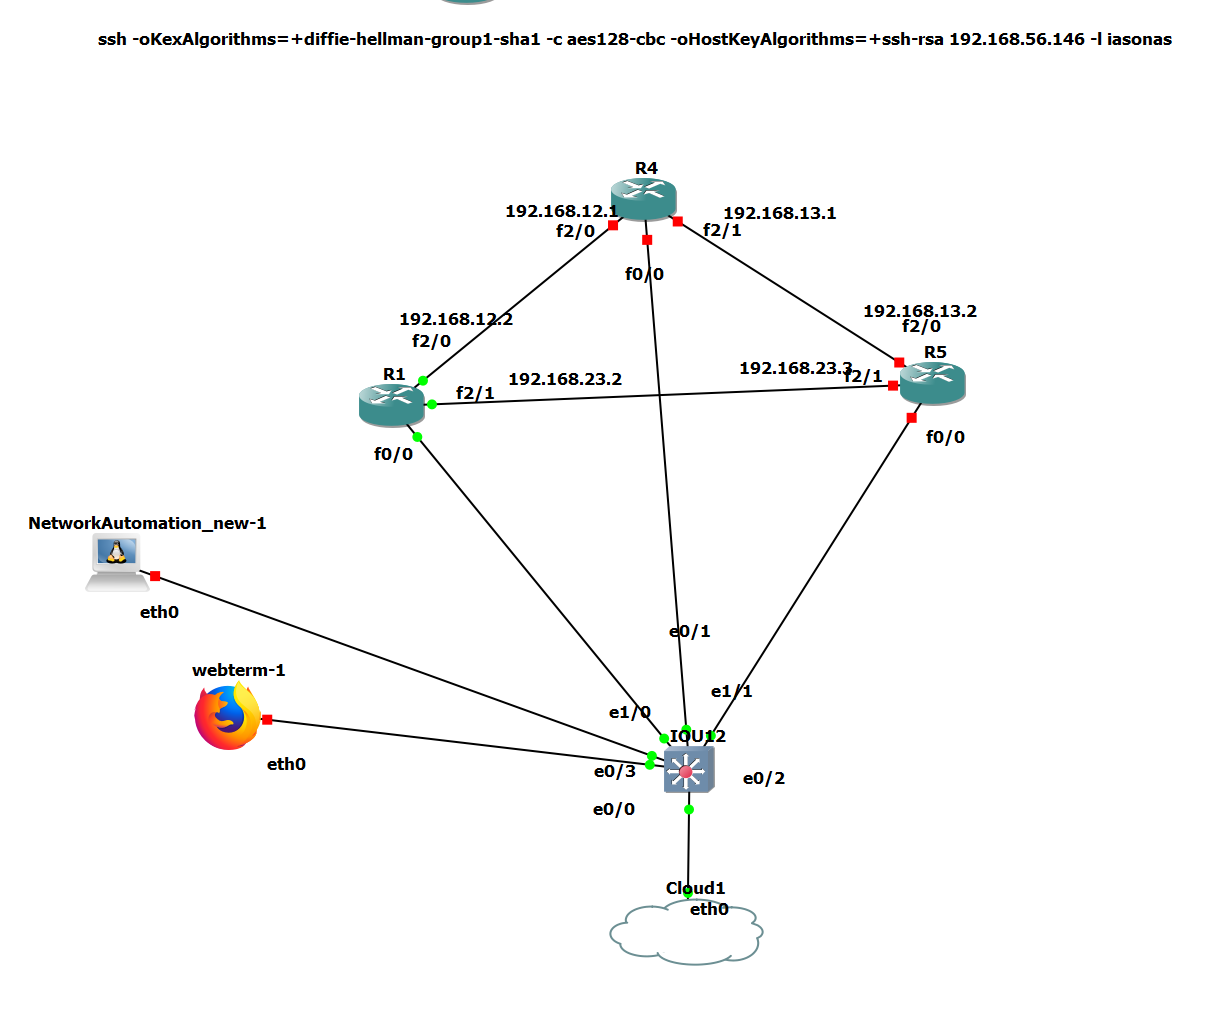
\includegraphics[width=0.7\textwidth]{graphics/Network_topology.png}
	\caption{\en{General Network Topology} }
\end{figure}



\section{\en{Cisco IOS}}

Το \en{IOU} είναι μια εικονική έκδοση του λογισμικού \en{IOS} της \en{Cisco} που 
μπορεί να χρησιμοποιηθεί για σκοπούς προσομοίωσης και δοκιμής δικτύου. Επιτρέπει στους μηχανικούς δικτύου να δημιουργούν εικονικές τοπολογίες δικτύου και να εξασκούνται σε διάφορες εργασίες δικτύου, 
όπως η διαμόρφωση δρομολογητών και μεταγωγέων, χωρίς να απαιτείται φυσικό υλικό. Το πλεονέκτημα του \en{GNS3} σε σχέση με εφαρμογές άλλες όπως το \en{Packet tracer} είναι ότι το \en{GNS3} 
μπορεί να σηκώσει πραγματικά \en{images} άρα πραγματικό λογισμικό συνεπώς οι λειτουργίες που μπορείς να κάνεις είναι πολύ περισσότερες.

Το \en{Cisco IOU}[20] χρησιμοποιείται συχνά σε συνδυασμό με λογισμικό προσομοίωσης δικτύου όπως 
\en{GNS3} ή \en{EVE-NG}, τα οποία αποτελούν την πλατφόρμα εικονικοποίησης δικτύου που σας επιτρέπει να 
να δημιουργείτε και να διαχειρίζεστε εικονικά περιβάλλοντα δικτύου για σκοπούς δοκιμής και εκμάθησης, τα οποία παρέχουν ένα γραφικό περιβάλλον χρήστη για τη δημιουργία και τη διαχείριση εικονικών 
τοπολογιών δικτύου. Οι εικόνες \en{IOU} μπορούν να φορτωθούν σε αυτά τα εργαλεία προσομοίωσης για τη δημιουργία εικονικών συσκευών \en{Cisco} που μπορούν να διαμορφωθούν και να δοκιμαστούν όπως το φυσικό δίκτυο 
συσκευές.

Το \en{IOS} μπορεί να τρέχει κατευθείαν πάνω σε υλικό, δηλαδή μπορεί 
να εγκατασταθεί απευθείας πάνω στα \en{router} και στα \en{switches} . 
Το \en{IOU} είναι λογισμικό το οποίο μπορεί να τρέξει το λογισμικό(\en{IOS})
ακόμα και σε \en{PC} προσομοιώνοντας με αυτόν τον τρόπο λογισμικό 
δικτυακών συσκευών χωρίς την ανάγκη ύπαρξης συγκεκριμένου υλικού.


\section{Εικονικοποίηση}
Στην επιστήμη της πληροφορικής, η εικονικοποίηση \en{virtualization} είναι ένας ευρύς όρος 
των υπολογιστικών συστημάτων που αναφέρεται σε έναν μηχανισμό αφαίρεσης, 
στοχευμένο στην απόκρυψη λεπτομερειών της υλοποίησης και της κατάστασης
ορισμένων υπολογιστικών πόρων από πελάτες των πόρων αυτών 
(π.χ. εφαρμογές, άλλα συστήματα, χρήστες κλπ). 
Η εν λόγω αφαίρεση μπορεί είτε να αναγκάζει έναν πόρο να 
συμπεριφέρεται ως πλειάδα πόρων (π.χ. μία συσκευή αποθήκευσης σε διακομιστή τοπικού δικτύου),
είτε πολλαπλούς πόρους να συμπεριφέρονται ως ένας (π.χ. συσκευές αποθήκευσης σε κατανεμημένα συστήματα). 

Η εικονικοποίηση δημιουργεί μία εξωτερική διασύνδεση η οποία αποκρύπτει την 
υποκείμενη υλοποίηση (π.χ. πολυπλέκοντας την πρόσβαση από διαφορετικούς χρήστες).
Αυτή η προσέγγιση στην εικονικοποίηση αναφέρεται ως εικονικοποίηση πόρων. 
Μία άλλη προσέγγιση, ίδιας όμως νοοτροπίας, είναι η εικονικοποίηση πλατφόρμας,
όπου η αφαίρεση που επιτελείται προσομοιώνει ολόκληρους υπολογιστές. Το αντίθετο της εικονικοποίησης είναι η διαφάνεια: 
ένας εικονικός πόρος είναι ορατός, αντιληπτός, αλλά στην πραγματικότητα ανύπαρκτος, 
ενώ ένας διαφανής πόρος είναι υπαρκτός αλλά αόρατος. 
 
Θα εξηγήσουμε την εικονικοποίηση στην δικιά μας περίπτωση. Το πρώτο επίπεδο είναι αυτό του υλικού. Η εικονικοποίηση
σα τεχνολογία εικονοποιεί το υλικό για να μπορέσει να δώσε πόρους στις εικονικές μηχανές. Η υλοιποίηση
της εικονικοποίησης γίνεται με λογισμικό \en{hypervisor}. Στη δικιά μας περίπτωση ο \en{hypervisor} είναι 
το \en{Virtual Box} ο οποίος είναι ένας τύπου Β \en{hypervisor}. Ο \en{hypervisor} τύπου 2 είναι μια εφαρμογή εγκατεστημένη 
στο λειτουργικό σύστημα του κεντρικού υπολογιστή το οποίο μας δίνει τη δυνατότητα να σηκώσουμε 
εικονικές μηχανές άλλων λειτουργικών συστημάτων πάνω στο ήδη υπάρχον σύστημα.

Οι παρακάτω εικόνες μπορούν να εξηγήσουν σχηματικά τη γενική καθώς και την ειδική αρχιτεκτονική.

\begin{figure}[htb]
	\centering
	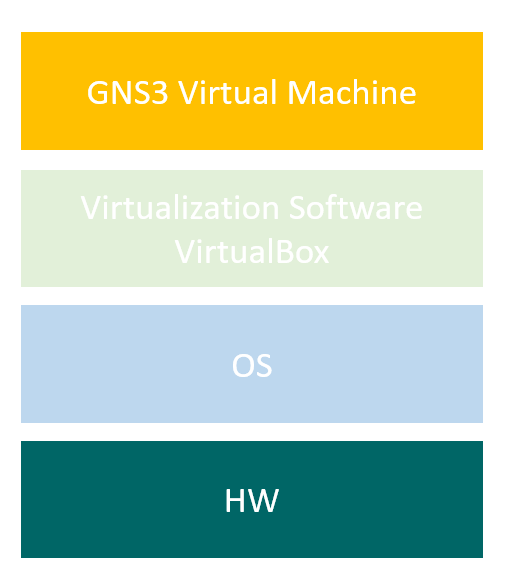
\includegraphics[width=0.5\textwidth]{graphics/Architecture_virtualbox.PNG}
	\caption{\en{Virtualization} Γενική αρχιτεκτονική}
\end{figure}

\begin{figure}[htb]
	\centering
	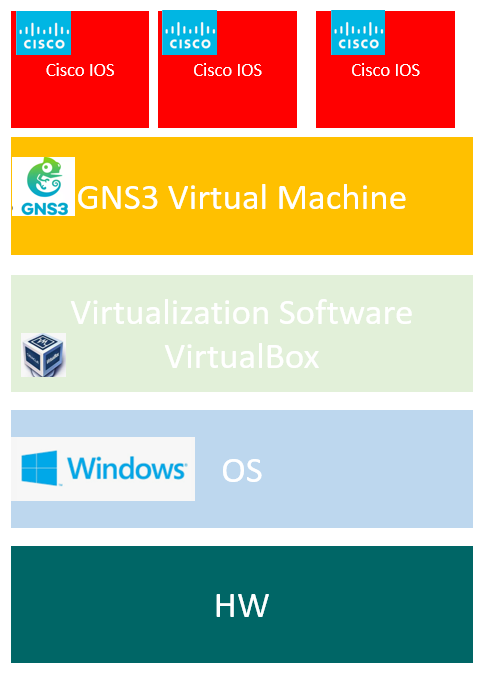
\includegraphics[width=0.5\textwidth]{graphics/virtualization_architecture.PNG}
	\caption{\en{Virtualization} Γενική αρχιτεκτονική}
\end{figure}

\section{Πρόγραμμα εικονοποίησης για το \en{GNS3 VM-VirtualBox}}

Το \en{Oracle VM VirtualBox} ή \en{VirtualBox} (πρώην en{Sun VirtualBox}, \en{Sun xVM VirtualBox} και \en{Innotek VirtualBox}) είναι υπερεπόπτης
ανοιχτού κώδικα για υπολογιστές \en{x86} που αναπτύσσεται από την \en{Oracle Corporation}.
Αναπτύχθηκε αρχικά από την \en{Innotek GmbH}
και αποκτήθηκε από τη \en{Sun Microsystems} το 2008, η οποία εξαγοράστηκε από την \en{Oracle} το 2010.

Το \en{VirtualBox} μπορεί να εγκατασταθεί σε διάφορα λειτουργικά συστήματα, συμπεριλαμβανόμενων των \en{Linux, macOS, Windows, Solaris} και \en{OpenSolaris}.
Υπάρχουν επίσης μεταφορές για το \en{FreeBSD} και το \en{Genode}.
Υποστηρίζει τη δημιουργία και τη διαχείριση εικονικών μηχανών που εκτελούν εκδόσεις και παραλλαγές των \en{Microsoft Windows, Linux, BSD, Solaris, Haiku, OSx86}
και άλλα, καθώς και περιορισμένη εικονικοποίηση \en{macOS}.
Για ορισμένα λειτουργικά συστήματα είναι διαθέσιμο ένα πακέτο \en{"Guest Additions"} από μηχανές συσκευών και εφαρμογές συστήματος
που συνήθως βελτιώνει την απόδοση, ειδικά των γραφικών. Επίσης δίνει την δυνατότητα στον χρήστη να μεταφέρει αρχεία ή κείμενο από μία εικονική μηχανή στον υπολογιστή του χρήστη και να αυξήσει την ανάλυση του παράθυρου της μηχανής. 
Στην εικόνα 3.4 μπορούμε να δούμε το \en{VirtualBox} και την εικονική μηχανή \en{GNS3 VM}

\begin{figure}[htb]
	\centering
	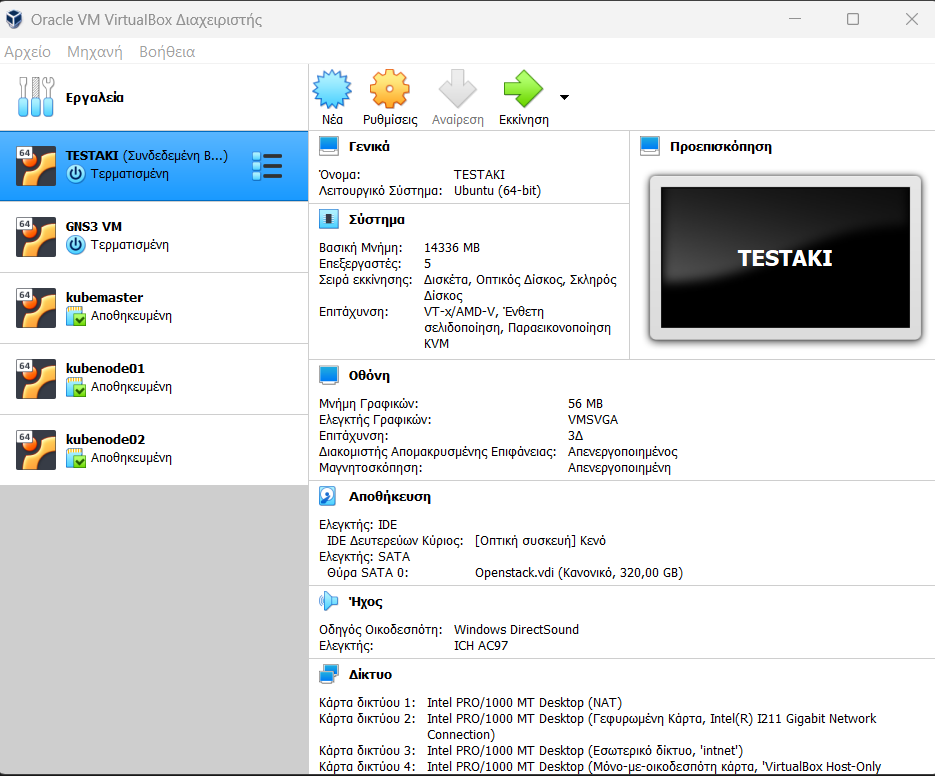
\includegraphics[width=0.9\textwidth]{graphics/virtualbox.PNG}
	\caption{\en{Virtualbox} }
\end{figure}

\section{\en{Django Web Framework}}

Το \en{Django} είναι ένα \en{backedn framework} το οποίο βασίζεται στη γλώσσα προγραμματισμού \en{Python}. Με το \en{Django}, μπορείτε να μεταφέρετε τις εφαρμογές Ιστού από την ιδέα στην κυκλοφορία μέσα σε λίγες ώρες. Το \en{Django} φροντίζει για μεγάλο μέρος
της ταλαιπωρίας της ανάπτυξης ιστού, ώστε να μπορείτε να εστιάσετε στη σύνταξη της εφαρμογής σας χωρίς να χρειάζεται να ανακαλύψετε ξανά τον τροχό.
Είναι δωρεάν και ανοιχτού κώδικα. Ορισμένες από τις πιο μεγάλες εταιρίες στον πλανήτη χρησιμοποιούν την ικανότητα του
να κλιμακώνεται γρήγορα και με ευελιξία για να ανταποκρίνεται στις μεγαλύτερες απαιτήσεις κίνησης. Στη δικιά μας περίπτωση χρησιμοποιήθηκε το συγκεκριμένου
{Framework} γιατί θα μας έδινε τη δυνατότητα να φτιάξουμε μία εφαρμογή με μεγάλη επεκτασιμότητα και παράλληλα να μπορέσουμε να ενσωματώσουμε μεσα διαφορετικές τεχνολογίες.

Παράλληλα με το \en{Django} χρησιμοποιήθηκαν έτοιμες βιβλιοθήκες της \en{Python} προκειμένου να μπορέσουν να εκτελεστούν βασικές λειτουργίες της εφαρμογής όπως 
τα πρωτοκολλα επικοινωνίας. Θεωρούμε ότι η δημιουργία τέτοιων βιβλιοθηκών ξεφεύγει από τα όρια μιας διπλωματικής εργασίας καθώς απαιτεί πολύ χρόνο και ερευνητική
ενασχόληση που μόνο στα πλαίσια ενός διδακτορικού θα μπορούσε να υλοποιηθεί μιά τέτοια ιδέα. Παρακάτων παρουσιάζονται οι βιβλιοθήκες που χρησιμοποιήθηκαν και κάποια βασικά χαρακτηριστικά τους.

\subsection{\en{Paramiko}}
Το \en{Paramiko}[21] είναι μια διασύνδεση καθαρά \en{Python} που υλοποιεί το πρωτόκολλο \en{SSH} έκδοσης 2 σε \en{Python}, παρέχοντας λειτουργικότητα τόσο πελάτη όσο και διακομιστή.
Το \en{Paramiko} μπορεί να επιτύχει υψηλές επιδόσεις σε χαμηλού επιπέδου κρυπτογραφικές έννοιες.
Οποιαδήποτε συσκευή που μπορεί να ρυθμιστεί μέσω \en{SSH} μπορεί επίσης να ρυθμιστεί από την \en{Python} με σενάρια με τη χρήση αυτής της μονάδας.

\subsection{\en{Netmiko}}
Το \en{Netmiko}[22] είναι μια βιβλιοθήκη ανοικτού κώδικα για πολλούς προμηθευτές, που σημαίνει ότι πολλές συσκευές μπορούν να ρυθμιστούν από την \en{python}
χρησιμοποιώντας το \en{Netmiko}.
Ορισμένες από τις συσκευές που υποστηρίζει το \en{Netmiko} είναι οι εξής: \en{Cisco IOS}, \en{Juniper}, \en{Arista}, \en{HP} και \en{Linux}. 
Μπορεί επίσης να υποστηρίζει και άλλους προμηθευτές όπως η \en{Alcatel}, η \en{Huawei} και η \en{Ubiquity} αλλά περιορισμένα 
δοκιμές έχουν γίνει με αυτούς τους προμηθευτές.
Το \en{Netmiko} τρέχει πάνω από το \en{Paramiko} για να κάνει τη σύνδεση \en{SSH} σε συσκευές δικτύου λιγότερο περίπλοκη, πιο ευέλικτη και πιο εύκολη στη χρήση. Παρόλο που το \en{Netmiko} είναι ευκολότερο στη χρήση, όπως αναφέρθηκε 
παραπάνω, υποστηρίζει συγκεκριμένους προμηθευτές και μόνο έναν αριθμό συσκευών τους. Από την άλλη πλευρά,
το \en{Paramiko} μπορεί να χρησιμοποιηθεί για την επικοινωνία με οποιαδήποτε συσκευή που υποστηρίζει \en{SSH}.
Τόσο το \en{Paramiko}όσο και το \en{Netmiko} αποτελούν εναλλακτικές επιλογές για συσκευές που δεν υποστηρίζουν 
\en{APIs}.

\subsection{\en{Napalm}}
Το \en{NAPALM}[23] (\en{Network Automation and Programmability Abstraction Layer with Multivendor support}) είναι μια βιβλιοθήκη \en{Python} που υλοποιεί ένα σύνολο λειτουργιών για την αλληλεπίδραση με διαφορετικά λειτουργικά συστήματα συσκευών δικτύου χρησιμοποιώντας ένα ενοποιημένο \en{API}.
Το \en{NAPALM} υποστηρίζει διάφορες μεθόδους σύνδεσης με τις συσκευές, χειρισμού των ρυθμίσεων ή ανάκτησης δεδομένων. Το \en{Napalm} συνεπώς είναι μια βιβλιοθήκη \en{Python} που παρέχει ένα \en{API}
\en{(Application Programming Interface)} για την εργασία με συσκευές δικτύου. Έχει σχεδιαστεί για να απλοποιεί την
αυτοματοποίηση και τη διαχείριση του δικτύου με την αφαίρεση των υποκείμενων λεπτομερειών που σχετίζονται με τον εκάστοτε προμηθευτή και την παροχή μιας συνεπούς διεπαφής σε διαφορετικά δίκτυα. 
συσκευών.
Το \en{Napalm} επιτρέπει στους μηχανικούς και τους διαχειριστές δικτύων να αυτοματοποιούν κοινές εργασίες διαχείρισης δικτύου, όπως η διαμόρφωση, η παροχή, η παρακολούθηση και η 
αντιμετώπιση προβλημάτων. Υποστηρίζει πολλούς προμηθευτές συσκευών δικτύου, συμπεριλαμβανομένων των \en{Cisco}, \en{Juniper}, \en{Arista} και \en{Huawei}.
Το \en{Napalm} παρέχει ένα σύνολο κοινών λειτουργιών που μπορούν να εκτελεστούν σε συσκευές δικτύου, όπως η ανάκτηση πληροφοριών διαμόρφωσης, η εφαρμογή διαμόρφωσης 
αλλαγών, έλεγχος στατιστικών στοιχείων διασύνδεσης και συλλογή πληροφοριών τοπολογίας δικτύου παρέχει επίσης χαρακτηριστικά όπως υποστήριξη επαναφοράς, επικύρωση διαμόρφωσης 
αλλαγών διαμόρφωσης, και σύγκριση των διαφορών διαμόρφωσης μεταξύ συσκευών.
14
Το \en{Napalm} μπορεί να συνδυαστεί με βιβλιοθήκες \en{Python} όπως οι \en{Netmiko}, \en{Paramiko} και \en{Ansible} για τη δημιουργία σύνθετων ροών εργασίας αυτοματισμού δικτύου. Μπορεί επίσης να ενσωματωθεί 
με δημοφιλή εργαλεία παρακολούθησης δικτύου, όπως το \en{Prometheus} και το \en{Grafana}, για την παρακολούθηση της απόδοσης του δικτύου σε πραγματικό χρόνο.

Η συνάρτηση \en{get_network_driver} της βιβλιοθήκης \en{NAPALM} 
χρησιμοποιείται στην εφαρμογή μας  προκειμένου το  \en{User Interface} 
του \en{Django}  να αποκτήσει έναν οδηγό δικτύου που επιτρέπει την 
αλληλεπίδραση με τις συσκευές της \en{Cisco} μέσω ενός ενιαίαου \en{API}. 
Αυτό διευκολύνει την αυτοματοποίηση και τη διαχείριση των συσκυεών 
χρησιμοποιώντας το πρωτόκολλο \en{SSH}.




